
\chapter{Feature Visualisation of Different Network Layers}
\label{appendix:feature_vis}
This appendix presents feature visualisation applied to different parts of the trained VBF DCNN model's convolutional section.
This is to demonstrate how features are constructed and combined as one goes deeper into the network starting with the spread layer.
Earlier layers are optimised for the mean over a feature map, later ones are for a single neuron as the receptive field becomes so large that trying to optimise them all does not show much structure.
The reader is referred to Figure \ref{fig:event_categorisation:vbf_dcnn_figure} for where the named places are located in the network.

These images are all normalised by dividing by the highest valued pixel in the dijet image. This will show the relative weighting of features from the leading vs subleading jet image channels.

\begin{figure}[h!]
    \begin{center}
        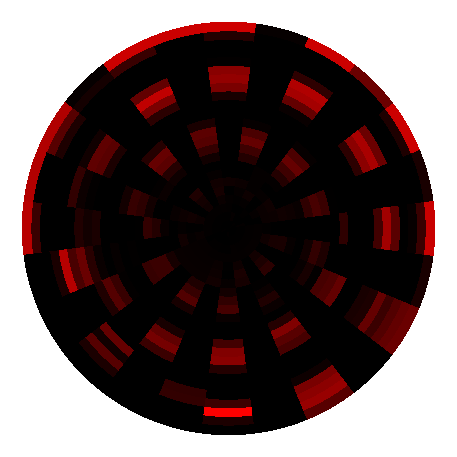
\includegraphics[width=0.32\textwidth]{figures/appendix_featurevis/spread_12.pdf}
        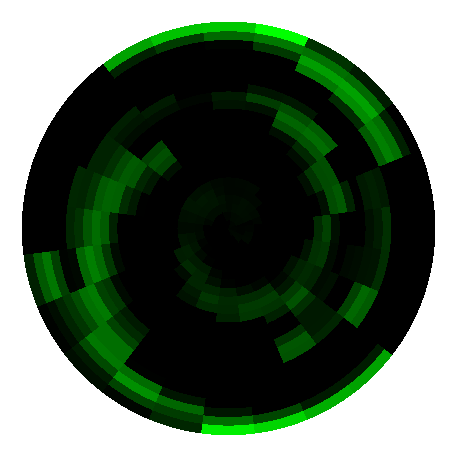
\includegraphics[width=0.32\textwidth]{figures/appendix_featurevis/spread_20.pdf}
        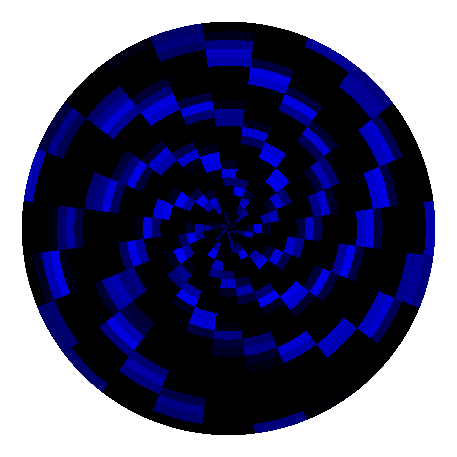
\includegraphics[width=0.32\textwidth]{figures/appendix_featurevis/spread_33.pdf}
    \end{center}
    \begin{center}
        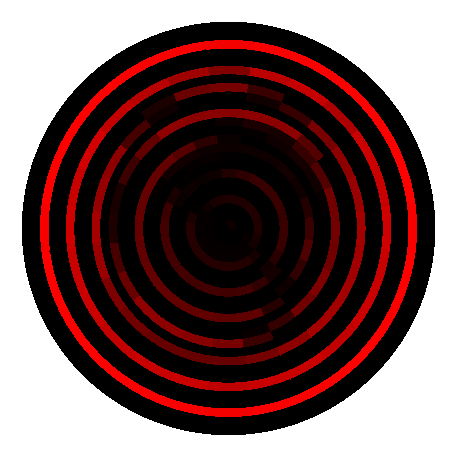
\includegraphics[width=0.32\textwidth]{figures/appendix_featurevis/spread_0.pdf}
        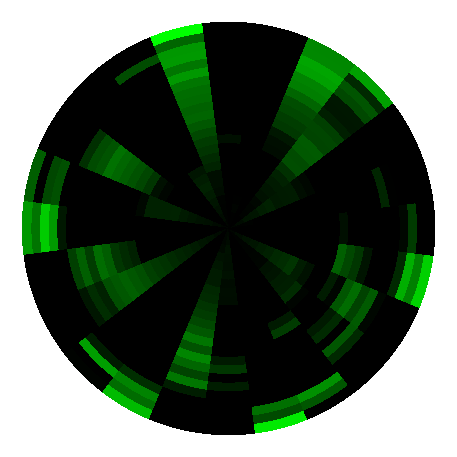
\includegraphics[width=0.32\textwidth]{figures/appendix_featurevis/spread_23.pdf}
        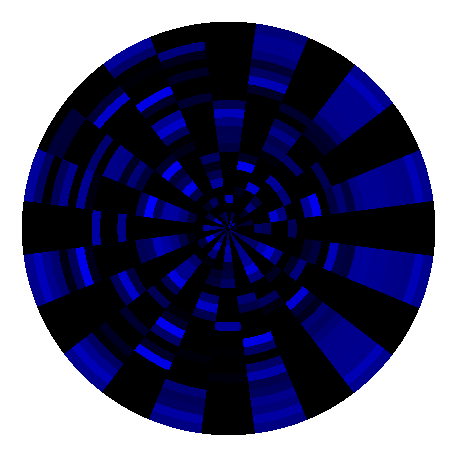
\includegraphics[width=0.32\textwidth]{figures/appendix_featurevis/spread_45.pdf}
    \end{center}
    \begin{center}
        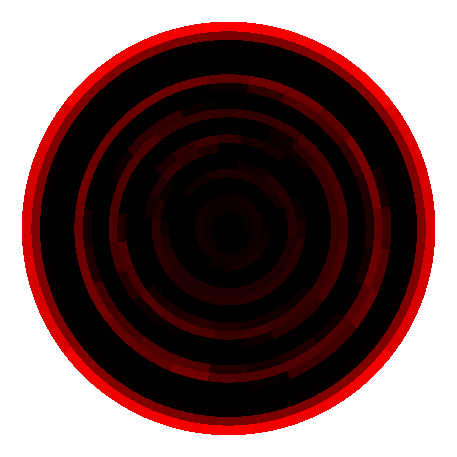
\includegraphics[width=0.32\textwidth]{figures/appendix_featurevis/spread_1.pdf}
        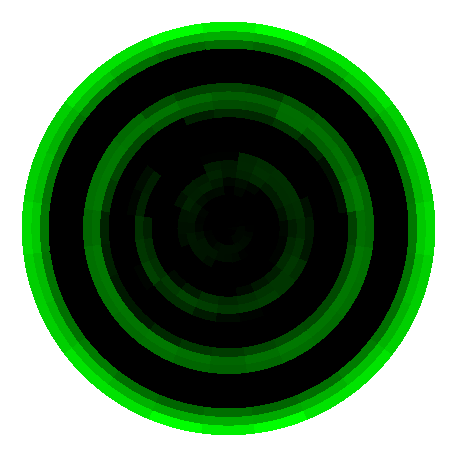
\includegraphics[width=0.32\textwidth]{figures/appendix_featurevis/spread_31.pdf}
        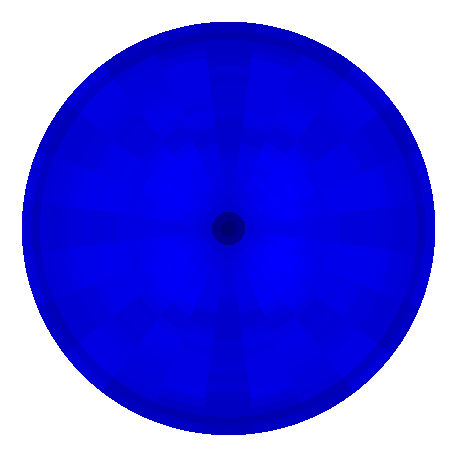
\includegraphics[width=0.32\textwidth]{figures/appendix_featurevis/spread_46.pdf}
    \end{center}
    \begin{center}
        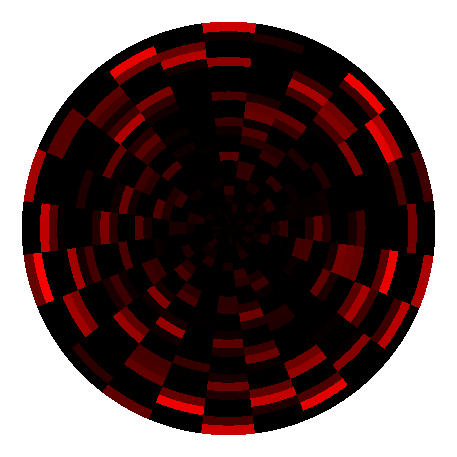
\includegraphics[width=0.32\textwidth]{figures/appendix_featurevis/spread_5.pdf}
        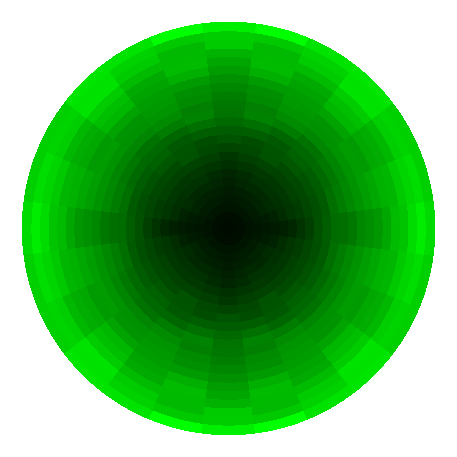
\includegraphics[width=0.32\textwidth]{figures/appendix_featurevis/spread_19.pdf}
        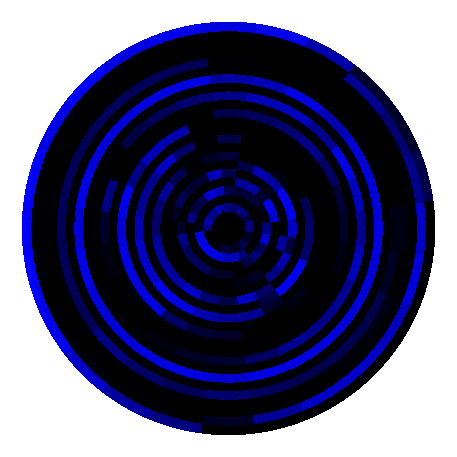
\includegraphics[width=0.32\textwidth]{figures/appendix_featurevis/spread_32.pdf}
    \end{center}
    \caption{Feature visualisation of the spread layer features. Red is the charged \pt channel, green is the neutral \pt channel
             and blue is the PF candidate multiplicity channel. This layer only constructs features in individual channels.
             Optimisation objective is the mean of the values over a whole feature map.}
\end{figure}

\begin{figure}[h!]
    \begin{center}
        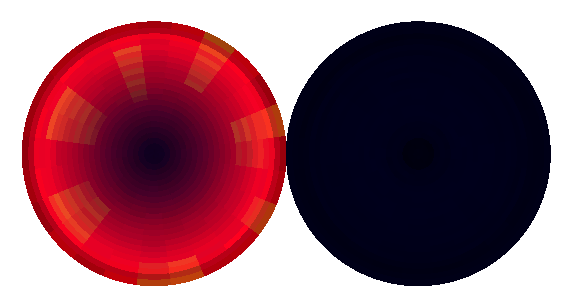
\includegraphics[width=0.49\textwidth]{figures/appendix_featurevis/TU1_9.pdf}
        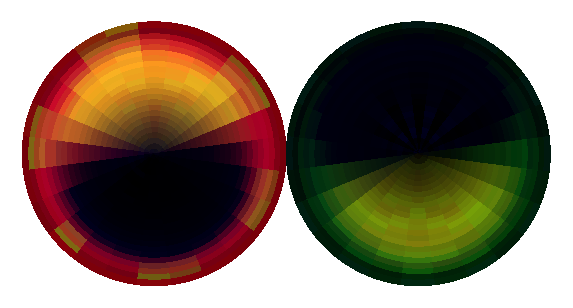
\includegraphics[width=0.49\textwidth]{figures/appendix_featurevis/TU1_10.pdf}
    \end{center}
    \begin{center}
        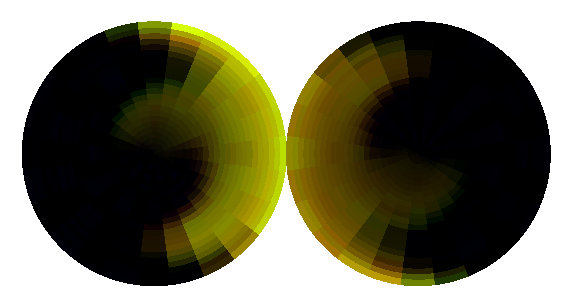
\includegraphics[width=0.49\textwidth]{figures/appendix_featurevis/TU1_37.pdf}
        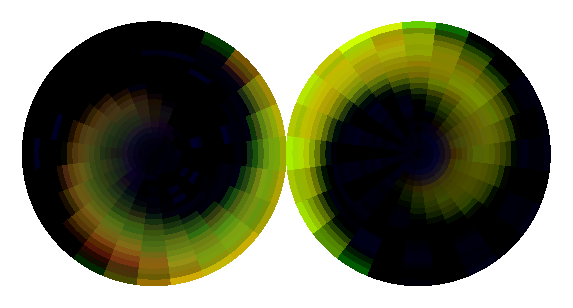
\includegraphics[width=0.49\textwidth]{figures/appendix_featurevis/TU1_45.pdf}
    \end{center}
    \begin{center}
        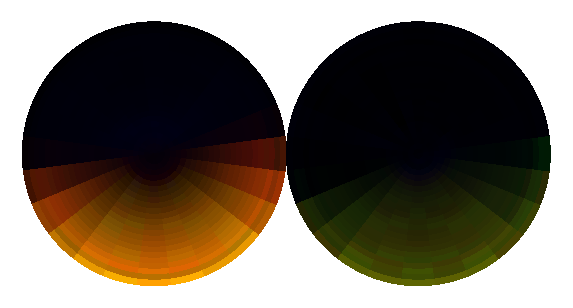
\includegraphics[width=0.49\textwidth]{figures/appendix_featurevis/TU1_55.pdf}
        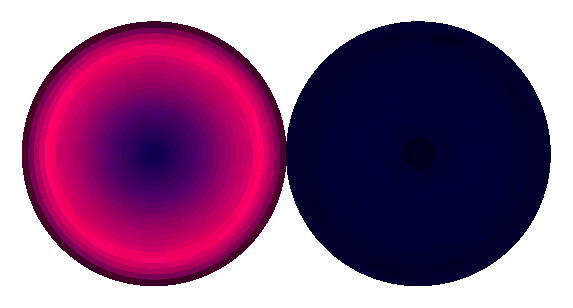
\includegraphics[width=0.49\textwidth]{figures/appendix_featurevis/TU1_40.pdf}
    \end{center}
    \begin{center}
        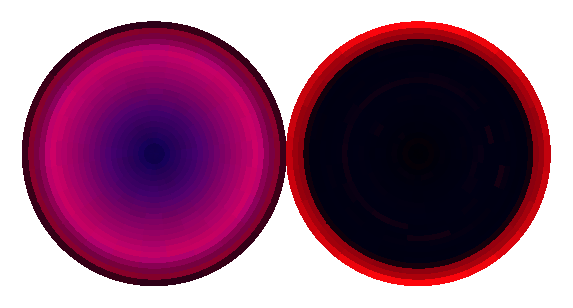
\includegraphics[width=0.49\textwidth]{figures/appendix_featurevis/TU1_8.pdf}
        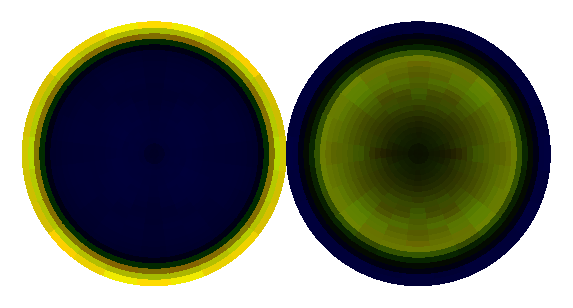
\includegraphics[width=0.49\textwidth]{figures/appendix_featurevis/TU1_27.pdf}
    \end{center}
    \caption{Feature visualisation of the output of TU1. Here the low level features have been combined together to compare structure across channels, 
             directly opposite around the jet axis and between the jets of the dijet.
             Optimisation objective is the mean of the values over a whole feature map.}
\end{figure}

\begin{figure}[h!]
    \begin{center}
        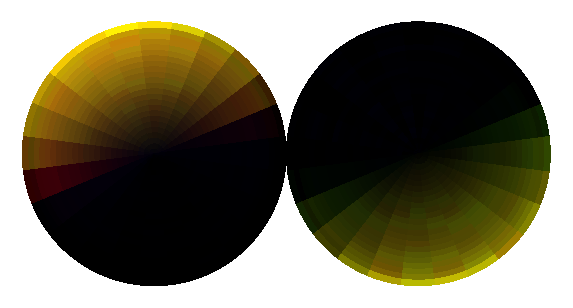
\includegraphics[width=0.49\textwidth]{figures/appendix_featurevis/TU2_20.pdf}
        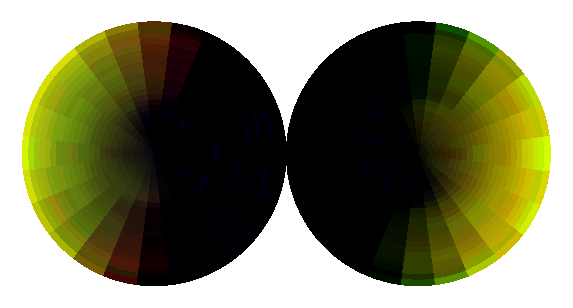
\includegraphics[width=0.49\textwidth]{figures/appendix_featurevis/TU2_24.pdf}
    \end{center}
    \begin{center}
        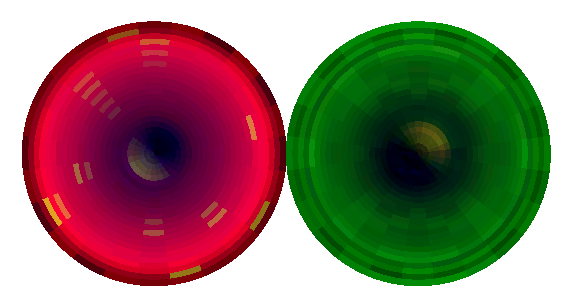
\includegraphics[width=0.49\textwidth]{figures/appendix_featurevis/TU2_3.pdf}
        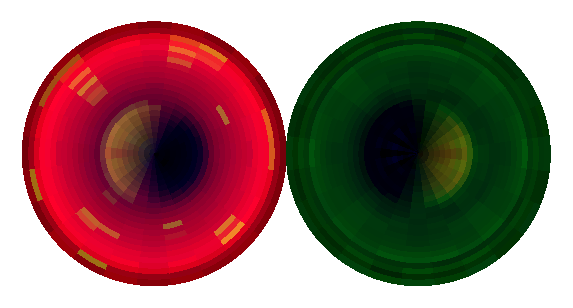
\includegraphics[width=0.49\textwidth]{figures/appendix_featurevis/TU2_21.pdf}
    \end{center}
    \begin{center}
        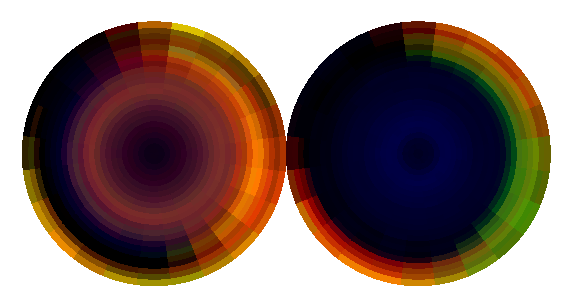
\includegraphics[width=0.49\textwidth]{figures/appendix_featurevis/TU2_28.pdf}
        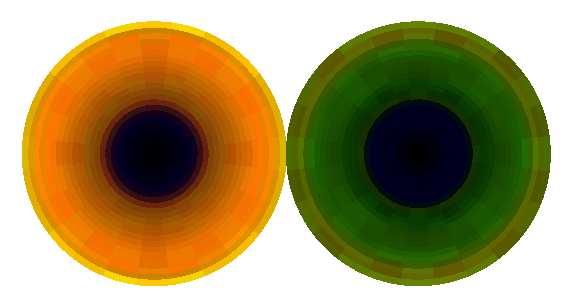
\includegraphics[width=0.49\textwidth]{figures/appendix_featurevis/TU2_6.pdf}
    \end{center}
    \begin{center}
        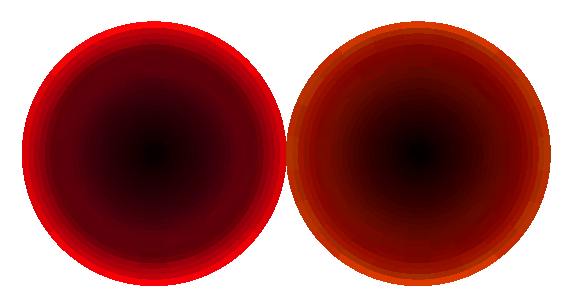
\includegraphics[width=0.49\textwidth]{figures/appendix_featurevis/TU2_0.pdf}
        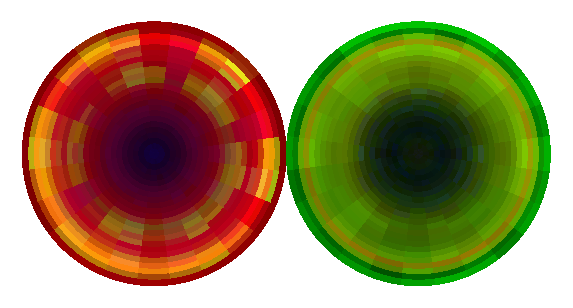
\includegraphics[width=0.49\textwidth]{figures/appendix_featurevis/TU2_41.pdf}
    \end{center}
    \caption{Feature visualisation of the output of TU2. Here the features of TU1 are combined to make more complex features, 
    but they are also reused (this is facilitated by the skip connections and is a capability of dense CNNs).
    Optimisation objective is the mean of the values over a whole feature map.}
\end{figure}

\begin{figure}[h!]
    \begin{center}
        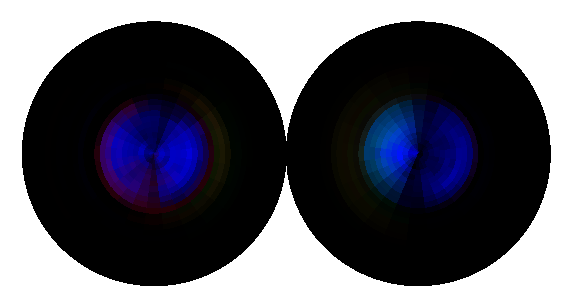
\includegraphics[width=0.49\textwidth]{figures/appendix_featurevis/TU3_0_1_0.pdf}
        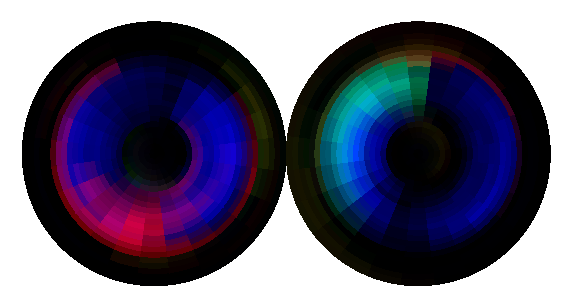
\includegraphics[width=0.49\textwidth]{figures/appendix_featurevis/TU3_0_1_1.pdf}
    \end{center}
    \begin{center}
        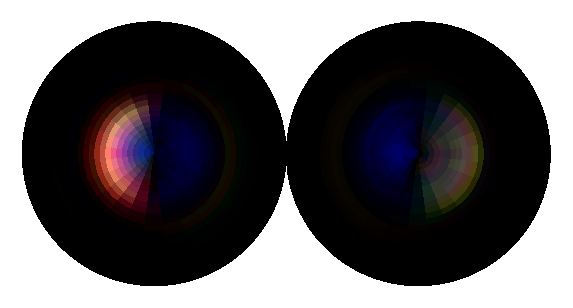
\includegraphics[width=0.49\textwidth]{figures/appendix_featurevis/TU3_3_1_0.pdf}
        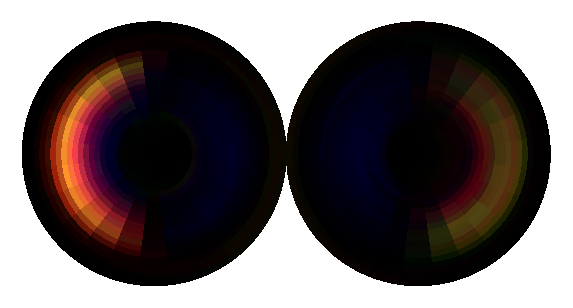
\includegraphics[width=0.49\textwidth]{figures/appendix_featurevis/TU3_3_1_1.pdf}
    \end{center}
    \begin{center}
        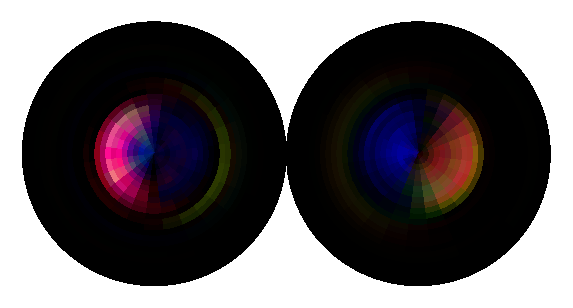
\includegraphics[width=0.49\textwidth]{figures/appendix_featurevis/TU3_4_1_0.pdf}
        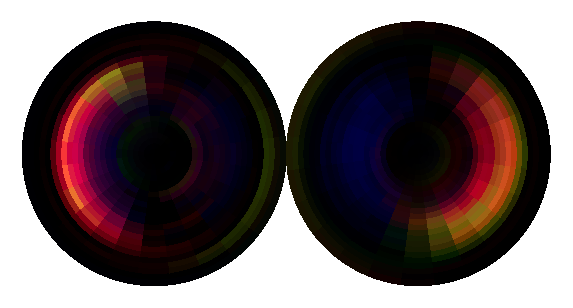
\includegraphics[width=0.49\textwidth]{figures/appendix_featurevis/TU3_4_1_1.pdf}
    \end{center}
    \begin{center}
        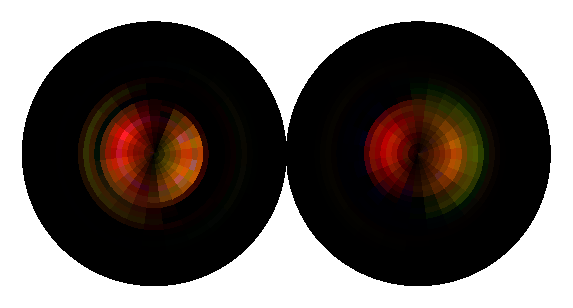
\includegraphics[width=0.49\textwidth]{figures/appendix_featurevis/TU3_6_1_0.pdf}
        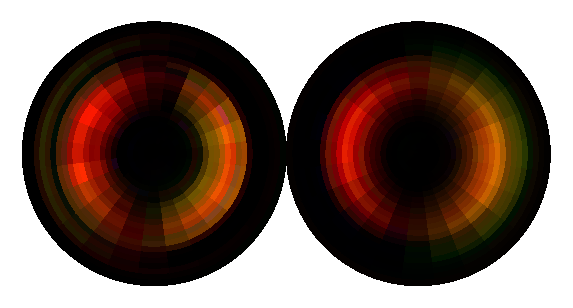
\includegraphics[width=0.49\textwidth]{figures/appendix_featurevis/TU3_6_1_1.pdf}
    \end{center}
    \caption{Feature visualisations of individual neuron values after TU3. These constitute the learned features used in the main discriminant.
             These images are optimised to maximally activate a single neuron rather than the mean of the neurons of one feature map.}
\end{figure}


